% Template for a Computer Science Tripos Part II project dissertation
\documentclass[12pt,a4paper,twoside,openright]{report}
\usepackage[pdfborder={0 0 0}]{hyperref}    % turns references into hyperlinks
\usepackage[margin=25mm]{geometry}  % adjusts page layout
\usepackage{graphicx}  % allows inclusion of PDF, PNG and JPG images
\usepackage{verbatim}
\usepackage{docmute}   % only needed to allow inclusion of proposal.tex

\raggedbottom                           % try to avoid widows and orphans
\sloppy
\clubpenalty1000%
\widowpenalty1000%

\renewcommand{\baselinestretch}{1.1}    % adjust line spacing to make
                                        % more readable

\begin{document}

\bibliographystyle{plain}


%%%%%%%%%%%%%%%%%%%%%%%%%%%%%%%%%%%%%%%%%%%%%%%%%%%%%%%%%%%%%%%%%%%%%%%%
% Title


\pagestyle{empty}

\rightline{\LARGE \textbf{Martin Richards}}

\vspace*{60mm}
\begin{center}
\Huge
\textbf{How to write a dissertation in \LaTeX} \\[5mm]
Computer Science Tripos -- Part II \\[5mm]
St John's College \\[5mm]
\today  % today's date
\end{center}

%%%%%%%%%%%%%%%%%%%%%%%%%%%%%%%%%%%%%%%%%%%%%%%%%%%%%%%%%%%%%%%%%%%%%%%%%%%%%%
% Proforma, table of contents and list of figures

\pagestyle{plain}

\chapter*{Proforma}

{\large
\begin{tabular}{ll}
Name:               & \bf Martin Richards                       \\
College:            & \bf St John's College                     \\
Project Title:      & \bf How to write a dissertation in \LaTeX \\
Examination:        & \bf Computer Science Tripos -- Part II, July 2001  \\
Word Count:         & \bf 1587\footnotemark[1]
                      (well less than the 12000 limit)  \\
Project Originator: & Dr M.~Richards                    \\
Supervisor:         & Dr Markus Kuhn                    \\ 
\end{tabular}
}
\footnotetext[1]{This word count was computed
by \texttt{detex diss.tex | tr -cd '0-9A-Za-z $\tt\backslash$n' | wc -w}
}
\stepcounter{footnote}


\section*{Original Aims of the Project}

To write a demonstration dissertation\footnote{A normal footnote without the
complication of being in a table.} using \LaTeX\ to save
student's time when writing their own dissertations. The dissertation
should illustrate how to use the more common \LaTeX\ constructs. It
should include pictures and diagrams to show how these can be
incorporated into the dissertation.  It should contain the entire
\LaTeX\ source of the dissertation and the makefile.  It should
explain how to construct an MSDOS disk of the dissertation in
Postscript format that can be used by the book shop for printing, and,
finally, it should have the prescribed layout and format of a diploma
dissertation.


\section*{Work Completed}

All that has been completed appears in this dissertation.

\section*{Special Difficulties}

Learning how to incorporate encapulated postscript into a \LaTeX\
document on both Ubuntu Linux and OS X.
 
\newpage
\section*{Declaration}

I, [Name] of [College], being a candidate for Part II of the Computer
Science Tripos [or the Diploma in Computer Science], hereby declare
that this dissertation and the work described in it are my own work,
unaided except as may be specified below, and that the dissertation
does not contain material that has already been used to any substantial
extent for a comparable purpose.

\bigskip
\leftline{Signed [signature]}

\medskip
\leftline{Date [date]}

\tableofcontents

\listoffigures

\newpage
\section*{Acknowledgements}

This document owes much to an earlier version written by Simon Moore
\cite{Moore95}.  His help, encouragement and advice was greatly 
appreciated.

%%%%%%%%%%%%%%%%%%%%%%%%%%%%%%%%%%%%%%%%%%%%%%%%%%%%%%%%%%%%%%%%%%%%%%%
% now for the chapters

\pagestyle{headings}

\chapter{Introduction}

\section{Overview of the files}

This document consists of the following files:

\begin{itemize}
\item \texttt{makefile} --- The makefile for the dissertation and
                         Project Proposal
\item \texttt{diss.tex} --- The dissertation
\item \texttt{proposal.tex}  --- The project proposal 
\item \texttt{figs} -- A directory containing diagrams and pictures
\item \texttt{refs.bib} --- The bibliography database
\end{itemize}

\section{Building the document}

This document was produced using \LaTeXe which is based upon
\LaTeX\cite{Lamport86}.  To build the document you first need to
generate \texttt{diss.aux} which, amongst other things, contains the
references used.  This if done by executing the command:

\texttt{pdflatex diss}

\noindent
Then the bibliography can be generated from \texttt{refs.bib} using:

\texttt{bibtex diss}

\noindent
Finally, to ensure all the page numbering is correct run \texttt{pdflatex}
on \texttt{diss.tex} until the \texttt{.aux} files do not change.  This
usually takes 2 more runs.

\subsection{The makefile}

To simplify the calls to \texttt{pdflatex} and \texttt{bibtex}, 
a makefile has been provided, see Appendix~\ref{makefile}. 
It provides the following facilities:

\begin{description}

\item\texttt{make} \\
 Display help information.

\item\texttt{make proposal.pdf} \\
 Format the proposal document as a PDF.

\item\texttt{make view-proposal} \\
 Run \texttt{make proposal.pdf} and then display it with a Linux PDF viewer
 (preferably ``okular'', if that is not available fall back to ``evince'').

\item\texttt{make diss.pdf} \\
 Format the dissertation document as a PDF.

\item\texttt{make count} \\
Display an estimate of the word count.

\item\texttt{make all} \\
Construct \texttt{proposal.pdf} and \texttt{diss.pdf}.

\item\texttt{make pub} \\ Make \texttt{diss.pdf}
and place it in my \texttt{public\_html} directory.

\item\texttt{make clean} \\ Delete all intermediate files except the
source files and the resulting PDFs. All these deleted files can
be reconstructed by typing \texttt{make all}.

\end{description}


\section{Counting words}

An approximate word count of the body of the dissertation may be
obtained using:

\texttt{wc diss.tex}

\noindent
Alternatively, try something like:

\verb/detex diss.tex | tr -cd '0-9A-Z a-z\n' | wc -w/


\chapter{Preparation}

This chapter is empty!


\chapter{Implementation}

\section{Verbatim text}

Verbatim text can be included using \verb|\begin{verbatim}| and
\verb|\end{verbatim}|. I normally use a slightly smaller font and
often squeeze the lines a little closer together, as in:

{\renewcommand{\baselinestretch}{0.8}\small
\begin{verbatim}
GET "libhdr"
 
GLOBAL { count:200; all  }
 
LET try(ld, row, rd) BE TEST row=all
                        THEN count := count + 1
                        ELSE { LET poss = all & ~(ld | row | rd)
                               UNTIL poss=0 DO
                               { LET p = poss & -poss
                                 poss := poss - p
                                 try(ld+p << 1, row+p, rd+p >> 1)
                               }
                             }
LET start() = VALOF
{ all := 1
  FOR i = 1 TO 12 DO
  { count := 0
    try(0, 0, 0)
    writef("Number of solutions to %i2-queens is %i5*n", i, count)
    all := 2*all + 1
  }
  RESULTIS 0
}
\end{verbatim}
}

\section{Tables}

\begin{samepage}
Here is a simple example\footnote{A footnote} of a table.

\begin{center}
\begin{tabular}{l|c|r}
Left      & Centred & Right \\
Justified &         & Justified \\[3mm]
%\hline\\%[-2mm]
First     & A       & XXX \\
Second    & AA      & XX  \\
Last      & AAA     & X   \\
\end{tabular}
\end{center}

\noindent
There is another example table in the proforma.
\end{samepage}

\section{Simple diagrams}

Simple diagrams can be written directly in \LaTeX.  For example, see
figure~\ref{latexpic1} on page~\pageref{latexpic1} and see
figure~\ref{latexpic2} on page~\pageref{latexpic2}.

\begin{figure}
\setlength{\unitlength}{1mm}
\begin{center}
\begin{picture}(125,100)
\put(0,80){\framebox(50,10){AAA}}
\put(0,60){\framebox(50,10){BBB}}
\put(0,40){\framebox(50,10){CCC}}
\put(0,20){\framebox(50,10){DDD}}
\put(0,00){\framebox(50,10){EEE}}

\put(75,80){\framebox(50,10){XXX}}
\put(75,60){\framebox(50,10){YYY}}
\put(75,40){\framebox(50,10){ZZZ}}

\put(25,80){\vector(0,-1){10}}
\put(25,60){\vector(0,-1){10}}
\put(25,50){\vector(0,1){10}}
\put(25,40){\vector(0,-1){10}}
\put(25,20){\vector(0,-1){10}}

\put(100,80){\vector(0,-1){10}}
\put(100,70){\vector(0,1){10}}
\put(100,60){\vector(0,-1){10}}
\put(100,50){\vector(0,1){10}}

\put(50,65){\vector(1,0){25}}
\put(75,65){\vector(-1,0){25}}
\end{picture}
\end{center}
\caption{A picture composed of boxes and vectors.}
\label{latexpic1}
\end{figure}

\begin{figure}
\setlength{\unitlength}{1mm}
\begin{center}

\begin{picture}(100,70)
\put(47,65){\circle{10}}
\put(45,64){abc}

\put(37,45){\circle{10}}
\put(37,51){\line(1,1){7}}
\put(35,44){def}

\put(57,25){\circle{10}}
\put(57,31){\line(-1,3){9}}
\put(57,31){\line(-3,2){15}}
\put(55,24){ghi}

\put(32,0){\framebox(10,10){A}}
\put(52,0){\framebox(10,10){B}}
\put(37,12){\line(0,1){26}}
\put(37,12){\line(2,1){15}}
\put(57,12){\line(0,2){6}}
\end{picture}

\end{center}
\caption{A diagram composed of circles, lines and boxes.}
\label{latexpic2}
\end{figure}



\section{Adding more complicated graphics}

The use of \LaTeX\ format can be tedious and it is often better to use
encapsulated postscript (EPS) or PDF to represent complicated graphics.
Figure~\ref{epsfig} and~\ref{xfig} on page \pageref{xfig} are
examples. The second figure was drawn using \texttt{xfig} and exported in
{\tt.eps} format. This is my recommended way of drawing all diagrams.


\begin{figure}[tbh]
\centerline{
\includegraphics{figs/cuarms.pdf}}
\caption{Example figure using encapsulated postscript}
\label{epsfig}
\end{figure}

\begin{figure}[tbh]
\vspace{4in}
\caption{Example figure where a picture can be pasted in}
\label{pastedfig}
\end{figure}


\begin{figure}[tbh]
\centerline{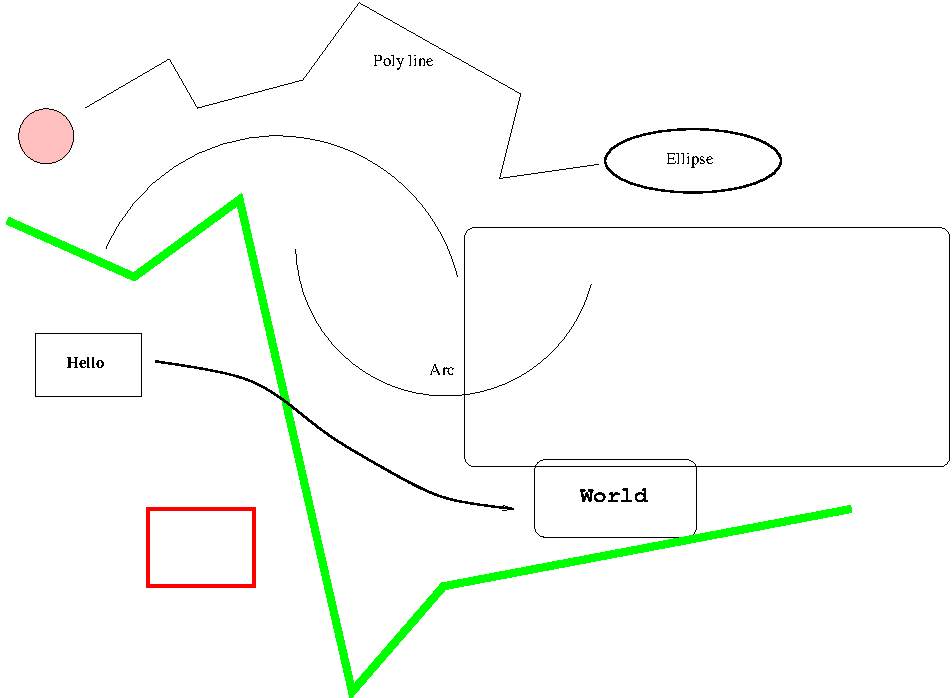
\includegraphics{figs/diagram.pdf}}
\caption{Example diagram drawn using \texttt{xfig}}
\label{xfig}
\end{figure}


\chapter{Evaluation}

\section{Printing and binding}

Use a ``duplex'' laser printer that can print on both sides to print
two copies of your dissertation. Then bind them, for example using the
comb binder in the Computer Laboratory Library.

\section{Further information}

See the Unix Tools notes at

\url{http://www.cl.cam.ac.uk/teaching/current-1/UnixTools/materials.html}


\chapter{Conclusion}

I hope that this rough guide to writing a dissertation is \LaTeX\ has
been helpful and saved you time.


%%%%%%%%%%%%%%%%%%%%%%%%%%%%%%%%%%%%%%%%%%%%%%%%%%%%%%%%%%%%%%%%%%%%%
% the bibliography
\addcontentsline{toc}{chapter}{Bibliography}
\bibliography{refs}

%%%%%%%%%%%%%%%%%%%%%%%%%%%%%%%%%%%%%%%%%%%%%%%%%%%%%%%%%%%%%%%%%%%%%
% the appendices
\appendix

\chapter{Latex source}

\section{diss.tex}
{\scriptsize\verbatiminput{diss.tex}}

\section{proposal.tex}
{\scriptsize\verbatiminput{proposal.tex}}

\chapter{Makefile}

\section{makefile}\label{makefile}
{\scriptsize\verbatiminput{makefile.txt}}

\section{refs.bib}
{\scriptsize\verbatiminput{refs.bib}}


\chapter{Project Proposal}

\vfil

\centerline{\Large Computer Science Project Proposal}
\vspace{0.4in}
\centerline{\Large Spectral Image Analysis for Medical Imaging}
\vspace{0.4in}
\centerline{\large M. Painter, Churchill College}
\vspace{0.3in}
\centerline{\large Originator: Dr. Pietro Lio'}
\vspace{0.3in}
\centerline{\large \date{\today}}

%\vfil


\noindent
{\bf Project Supervisor:} Dr Pietro Lio', Dr Gianluca Ascolani
\vspace{0.2in}

\noindent
{\bf Director of Studies:} Dr John Fawcett
\vspace{0.2in}
\noindent
 
\noindent
{\bf Project Overseers:} Prof John Daugman \& Dr David Greaves


% Main document
% ------------------------------------------------------------------------------

\section*{Introduction and Description of the Work}
The core idea of the project is to use spectral algorithms and machine learning 
to analyse biomedical images. I will explore the use of multiple learning 
techniques (namely Random Decision Forests and Neural Networks) and compare them 
via a number of metrics, described later. \\

The aim of the project will be to build a classifier that is capable of handling 
a wide variety of noisy medical images. Different types of medical images 
will present different challenges such as contrast between tissues and amount 
and type of noise. It will classify images per pixel into classes (dependent on 
the image), using the spectral analysis. \\

During the implementation I will start by implementing something for a toy 
problem, by which I mean an artificially produced, noiseless image. From this 
solution I will move onto solving the same problem with the introduction of 
artificial noise, at which point I will explore the use of de-noising 
techniques to improve the accuracy of the classifier. Finally after this I will 
move onto an implementation for real images. \\

For the real images I will use MRI images from Zhongzhao Teng from the Department 
of Radiology, Engineering, which include fatty tissues from patients with 
atherosclerosis (the build up of fatty tissues in arteries). In this case I can 
train the classifier to recognise regions of calcium, lipids, haemorragic tissue, 
and mixtures of these. \\

To demonstrate the versatility of the tool I will also use another set of images 
obtained in a completely different way, so will present a different set of 
challenges including the nature of noise in the image. The images are from Siri 
Luthman of the BSS group in the Department of Physics, and are obtained using a 
hyper-spectral camera with 72 spectral bins. The images use contrast agents with 
various spectral profiles, each of which has a negative binding response or 
neutral binding response for cancerous cells. By `negative binding response' I 
mean that the contrast agent binds to only non-cancerous cells, and `neutral' 
means that it binds to both cancerous and non-cancerous cells. Here the classes 
will be cancer cells, non-cancerous cell, and a mixture of both.







% The core of the project will perform spectral analysis of images and use this 
% for classifying images.

% -Explore spectral analysis of noisy images
% -Will compare different algorithms
% -MRI is about art....
% -Siri has provided images and I will do spectral analysis on it
% -Why do different image sets?
% - Diff types of noise - one is MRI
% - Medical images give many different challenges, diff data and diff ammount of noise, different contrasts between tissues.
% - Represent different challenges
% - See if can be adaptive enough to solve challenges of both images
% - Using specral methods - fourier transform and wavelets
%             - machine learning like random forests
% - different types of image with different 

% - de-noise and classify
%         - teng slideshow
%         - siri slideshow
%             -say what they are doing

% - neural networks and deep learning 
% - scrap GPU
% extension use machine learning and deep learning


% - give them something that describes the images for them.

% take some stuff from books and slides and not just siri
%         - not too much siri, physics and cl `speak diff languages'

% ---- What is the point?

% - don't talk about extension in intro, it has own section

% -diff noise from diff types of measurement and different techniques

% - meanwhile i will use to use these methods



% -start with an easy benchmark -> red circle on a black background
%                               -> standard benchmarks
%                               -> then add noise
%                               -> then move to medical images

%                               -> see anything interesting put into file.
%                               -> Pietro send lots of material, when see something interesting and then ask for the code if it's interesting.





% The core project is to implement a classifier of spectral images using a 
% machine learning algorithm, more specifically for use with medical imaging. I 
% will look at using different machine learning algorithms during my research 
% phase, and will implement at least one of these. \\

% In many medical images only some regions contain the cells/tissues that we are 
% interested in, so it would be useful to have a tool to indicate which regions 
% are of interest when teaching the machine. \\

% From some initial reading it appears that I may wish to use the Random 
% Forests algorithm, but this is something that I will want to look into further 
% at the beginning of my project. \\

% The system will initially just classify images as ``X'' is present in the image. 
% And hopefully if time will be able to indicate the regions of the image where 
% ``X'' is present. \\

% There will be many `endmembers' that will contribute to each pixels spectrum 
% seen in any medical image and so it is useful to be able to classify what might 
% be contained in each pixel. As I will be classifying per pixel it may be 
% amenable to GPU programming (which I will leave as an extension).



% ------------------------------------------------------------------------------

\section*{Starting Point}

I will use Java for the implementation of my algorithms and use libraries 
provided for Java. I will also use OpenCV's machine learning library as a 
benchmark to test my implementations against. 



% ------------------------------------------------------------------------------

\section*{Resources Required}

I will use my own computer to code on as I am more comfortable with it than the 
MCS machines. \\

I will also need example (spectral) image sets to be used in training and 
testing. I have kindly been provided with some MR images by Zhongzhao Teng of 
the Department of Ragiology and some hyperspectral images from Siri Luthman of 
the BSS group in the Department of Physics, as mentioned in the introduction.



% ------------------------------------------------------------------------------

\section*{Backup Plan}

I will be using a git repository for my project, which will be a private 
repository on GitHub. I will have two branches (at least, more if necessary) one 
`master' for completed features and one `in progress'. The in progress branch 
will be to push regularly any unfinished/in progress work onto so that my work 
is always backed up, and I don't loose any work in progress. \\

The local folder will also be in my Google Drive folder and so will be 
automatically synced to the Google servers, and I also have a time machine 
set up, which will take backups of the whole file system every hour.




% ------------------------------------------------------------------------------

\section*{Work to be done}

I can break down the project into the following stages:

\begin{enumerate}

\item 
Implement the infrastructure (data structures etc) and reading in of the raw
data.

\item 
Create a tool used to indicate areas of interest on the teaching data to be used 
with the training data.

\item 
Implement the main machine learning algorithm(s), and implement an out the 
box solution, initially to solve the `toy problem'. 

\item 
Extend the implementation to work for noisy images and then real images.

\end{enumerate}



% ------------------------------------------------------------------------------

\section*{Success Criterion for the Main Result}

I will use an `out the box' solution (such as OpenCV's machine learning 
libraries) as a benchmark to compare my implementation(s) against. I 
will provide each machine learning algorithm with the same inputs for training 
and the same inputs for testing and will use the following metrics to compare 
the performance of the systems and which has `learnt' better:
\begin{itemize}
    \item Overall run time (of classifying a single image);
    \item Accuracy of classifier (percentage images correctly identified).
\end{itemize}



% ------------------------------------------------------------------------------

\section*{Possible Extensions}

\begin{itemize}

    \item
    {\em Image Segmentation.}

    It would be useful to be able to segment the images given into separate 
    regions of interest. (For example if we want to classify an image with 
    cancer cells present, we indicate the regions containing cancerous cells).
    This is opposed to just returning the output per pixel, and would provide 
    a more useful output for users.

    \item 
    {\em Dimensionality Reduction.}

    If I finish the core of my project then one of the additional tasks that I 
    could look at would be to implement a data reduction (learning) algorithm. 
    In a spectral image with a high number of spectral bands it would be useful 
    to identify which spectral bands are important to the classification and 
    which are not. \\

    This problem more generally is called ``dimensionality reduction'' as we are 
    looking to reduce the dimension of data input to the algorithm.

\end{itemize}



% ------------------------------------------------------------------------------
% Put the timetable on a separate page so that we can print it out
\clearpage
\section*{Timetable: Workplan and Milestones to be achieved.}

% - - - - - 
{\bf Michaelmas weeks 3--4 (26th Oct to 4th Nov)} 

In preparation for the main implementation I will read about many machine 
learning algorithms. For example I will use the book ``Decision Forests for 
Computer Vision and Medical Image Analysis'' to learn about Random Forests. I 
will similarly research about Neural networks, and I will also research some 
other forms of learning algorithm. \\

{\em Deliverables:} 
\begin{itemize} 
    \item 
    A small description/overview of random forests and how they work, and a 
    similar description for any other learning algorithms researched. This 
    should be written up in \LaTeX\ for easy embedding into the preparation 
    chapter of the dissertation.
\end{itemize}

{\em Milestones:}
\begin{itemize}
    \item 
    Preparation reading completed, so that I am sufficiently able to implement 
    the learning algorithm(s) and handed in description of reading to project 
    supervisor for review - 4th Nov.
\end{itemize}



% - - - - - 
{\bf Michaelmas weeks 5--6 (5th Nov to 18th Nov)} 

I will spend this block familiarising myself with any technologies that I will 
possibly use. This will include the OpenCV library. I will also 
design a simple UI that will be used for the supervised learning. I will also 
familiarise myself with OpenCL and GPU programming. \\

{\em Deliverables:} 
\begin{itemize} 
    \item 
    A sketch of the UI for the tool which will be used for the supervised 
    learning.
    \item 
    A small overview of what OpenCV, GPU programming (or other technology(s) I 
    have looked at), and a description of why/where they will be useful. This 
    should again be written up in \LaTeX\ for easy embedding into the 
    preparation chapter of the dissertation.
\end{itemize}

{\em Milestones:}
\begin{itemize}
    \item 
    Handed in the UI design to supervisor for review - 9th Nov
    \item 
    Handed in the description of familiarisation of technologies to supervisor 
    for review - 18th Nov.
    \item 
    Demonstrated any small programs written for familiarisation to supervisor - 
    18th Nov.
\end{itemize}




% - - - - - 
{\bf Michaelmas weeks 7--8 (19th Nov to 2nd Dec)} 

{\em Implementation block 1}. Implement the infrastructure that will be used for 
the project. This will include loading the raw data into the appropriate data 
structures and do so efficiently as possible. \\

{\em Deliverables:} 
\begin{itemize} 
    \item 
    A bullet point list indicating what has been implemented during this block. 
    Written up in \LaTeX\ and to be used as a basis for the implementation 
    portion of the dissertation. To be handed in for review.
\end{itemize}

{\em Milestones:}
\begin{itemize}
    \item 
    Have the framework that I will use completed, including unit tests, and 
    demonstrate the tests to supervisor to check that this has been done - 2nd 
    Dec.
\end{itemize}




% - - - - - 
{\bf Christmas vacation weeks 1--2 (3rd Dec - 16th Dec)} 

I will be on holiday during this period and so I will work on little bits 
when I can, this may be catching up on any work that I got behind on in 
Michaelmas term (effectively making this a `slack' block), and I will begin 
some work on the next block if up to date. \\






% - - - - - 
{\bf Christmas vacation weeks 3--4 (17th Dec - 30th Dec)} 

{\em Implementation block 2}. Write the tool that will be used to indicate 
which images (or image regions) belong to a given class to be used for the 
supervised learning. \\

{\em Deliverables:} 
\begin{itemize} 
    \item 
    A bullet point list indicating what has been implemented during this block. 
    Written up in \LaTeX\ and to be used as a basis for the implementation 
    portion of the dissertation.
\end{itemize}

{\em Milestones:}
\begin{itemize}
    \item 
    Sent the completed tool to my supervisor as proof of completion. (As it is 
    the vacation I will not be in Cambridge and so will not be able to 
    demonstrate in person). - 30th Dec
\end{itemize}




% - - - - - 
{\bf Christmas vacation weeks 5--6 (31st Dec - 13th Jan)} 

{\em Implementation block 3}. Implement the machine learning algorithm(s) 
chosen, and also write the `out of the box' solution using the OpenCV 
library. At this stage I will only aim to have  \\

If this block is delivered on time then I am close to having a completed 
project. I have purposely stacked more of the work in the holiday compared to 
term time, as I have other commitments in term than out of term, such as 
lectures and supervisions. \\

{\em Deliverables:} 
\begin{itemize} 
    \item 
    A bullet point list indicating what has been implemented during this block. 
    Written up in \LaTeX\ and to be used as a basis for the implementation 
    portion of the dissertation.
\end{itemize}

{\em Milestones:}
\begin{itemize}
    \item 
    Finished writing the machine learning algorithm, and demonstrated it 
    classifying some `toy images' to supervisor - 13th Jan. (I will be back in 
    Cambridge by this time).
\end{itemize}




% - - - - - 
{\bf Lent weeks 1--2 (14th Jan - 27th Jan)} 

The progress report needs to be given up by noon on the 29th Jan, and so should 
be written in this block. \\

This rest of this block will be kept free for `slack'. This slack should include 
incorporating any feedback from my supervisor. \\

If I am up to date and there is no additional feedback that needs to be resolved, 
then I will proceed to work a block ahead. This will give me an additional block 
at the end of lent to implement any extensions. \\

{\em Deliverables:} 
\begin{itemize} 
    \item 
    Progress report.
    \item 
    Item written in \LaTeX\ which begins with the supervisors comments/feedback 
    and ends with how that was incorporated into the system.
\end{itemize}

{\em Milestones:}
\begin{itemize}
    \item 
    Demonstration of any features added made to supervisor - 27th Jan
\end{itemize}




% - - - - - 
{\bf Lent weeks 3--4 (28th Jan - 10th Feb)} 

{\em Implementation block 4}. In this block I will finish implementing my 
solution, and extend my simple solution to a more complex one capable of 
handling `toy images' with artificial noise, and then real images. This will 
require implementing de-noising of the images. \\

Also after the progress report a small presentation needs to be prepared. I 
will use the beginning of this time block to do this. \\

{\em Deliverables:} 
\begin{itemize} 
    \item 
    A bullet point list indicating what has been implemented during this block. 
    Written up in \LaTeX\ and to be used as a basis for the implementation 
    portion of the dissertation.
\end{itemize}

{\em Milestones:}
\begin{itemize}
    \item 
    Hand in progress report (completed in the previous block) - 29th Jan.
    \item 
    Perform a small mock presentation/interview with supervisor - 3rd Feb.
    \item 
    Made progress presentation to overseer group - ~5th Feb.
    \item 
    Finished implementing any de-noising algorithms, and have a working solution 
    for real images, including a demonstration to supervisor - 10th Feb.
\end{itemize}




% - - - - - 
{\bf Lent weeks 5--6 (11th Feb - 24th Feb)} 

Evaluation of the system. This will require writing tests that will gather 
the quantitative data (run time and accuracy of classification) to be used in 
the comparison required to satisfy the success criteria.\\

I will generate graphs from data in this phase using MATLAB, so that I can 
decide if the data is useful or not. This will prevent me from realising that 
the data isn't good at too late a stage in the project and when there is not 
enough time to re-evaluate the system. This has the advantage that the graphs 
will be ready to be exported directly into the dissertation. \\

{\em Deliverables:} 
\begin{itemize} 
    \item 
    Table for any qualitative data evaluated and spreadsheet of quantitative 
    data, which must include values for accuracy of the system (in a specific 
    test case) and timings for how long classification takes (on my home 
    machine).
    \item 
    Generated meaningful graphs using MATLAB with data gathered from evaluation.
\end{itemize}

{\em Milestones:}
\begin{itemize}
    \item 
    Table/spreadsheet completed and filled out with all data required for a good 
    write up. Spreadsheet and graphs sent to supervisor for reviewing - 24th Feb.
\end{itemize}




% - - - - - 
{\bf Lent weeks 7--8 (25th Feb - 9th Mar)} 

I will use my last block of work in lent as another `slack' block for if I get 
behind on any work for any reason such as a high load of supervision work 
through the term. This should also be used to incorporate any final feedback 
from my supervisor. \\

If am up to date at this point  I will work on implementing some of the 
extension tasks outlined in this document.

{\em Milestones:}
\begin{itemize}
    \item 
    System complete, success criterion met and demonstrated these to supervisor 
    - 9th Mar.
\end{itemize}




% - - - - - 
{\bf Easter vacation weeks 1--2 (10th Mar - 23rd Mar)} 

Set up the dissertation document and write introduction and preparation 
chapters of the dissertation. \\

{\em Deliverables:} 
\begin{itemize} 
    \item 
    Introduction and preparation chapters of dissertation.
\end{itemize}

{\em Milestones}: 
\begin{itemize}
    \item 
    Completed first draft of introduction chapter and given to supervisor 
    - 17th Mar.
    \item 
    Completed first draft of preparation chapter and given to supervisor 
    - 23rd Mar.
\end{itemize}




% - - - - - 
{\bf Easter vacation weeks 3--4 (24th Mar - 6th Apr)} 

Write up the implementation and evaluation chapters of the dissertation. \\

{\em Deliverables:} 
\begin{itemize} 
    \item 
    Implementation and evaluation chapters of dissertation.
\end{itemize}

{\em Milestones:}
\begin{itemize}
    \item 
    Completed first draft of implementation chapter and given to supervisor 
    - 31st Mar.
    \item 
    Completed first draft of the evaluation chapter and given to supervisor 
    - 6th Apr.
\end{itemize}




% - - - - - 
{\bf Easter vacation weeks 5--6 (7th Apr - 20th Apr)} 

Complete dissertation by completing the conclusion section and any appendices. 
I will also re-iterate through dissertation see if anything can be improved. \\

{\em Deliverables:} 
\begin{itemize} 
    \item 
    Draft of complete dissertation.
    \item 
    2nd draft of complete dissertation.
\end{itemize}

{\em Milestones:}
\begin{itemize}
    \item 
    Full first draft of dissertation handed into supervisor for review - 11th 
    Apr.
    \item 
    Hand in second draft of completed dissertation to supervisor - 18th Apr.
\end{itemize}


% - - - - - 
{\bf Easter term weeks 1--2 (21st Apr - 5th May)}  

Final `slack' block for the dissertation. If the dissertation is completed then 
I will proof read multiple times. I would like to have the dissertation 
`finished' by now to focus on revision for the exam and on learning any of the 
Easter term courses. \\

{\em Milestones:}
\begin{itemize}
    \item 
    System complete and success criterion met - 5th May.
\end{itemize}



% - - - - - 
{\bf Easter term week 3 (6th May - 13th May)} 

Final proof read and then an early submission so that I can focus on exam 
revision for the remainder of the term. \\

{\em Deliverables:} 
\begin{itemize} 
    \item 
    Dissertation.
\end{itemize}

{\em Milestones:}
\begin{itemize}
    \item 
    Hand in dissertation on time. (Project finished). - 13th May.
\end{itemize}




\end{document}
